
\subsection{Overview}
In response to the pilot results, we reconsider the data collection pipeline. 
We examined existing sketch datasets to see how their annotations could facilitate our data collection (dataset details are explained in Section \ref{relatedWorkChapter}).    
To shorten the time spent on sketching, we no longer asked annotators to sketch and instead only asked them to describe sketches in the QuickDraw dataset. Although we were no longer able to design text prompts ourselves and collect creative sketches like the ones in the previous pilot, we solved the problem that it was difficult to understand how some sketches illustrate the give prompts. 

The most important objective that this dataset should fulfill is allowing us to study how sketches share similar semantic parts and descriptions that are adapted to be used for different objects. Therefore, we must resolve the issue that some text descriptions we collected in the pilot either did not describe everything drawn in a step or described more than what was drawn.  
% To solve this problem of misaligned text descriptions and drawings, 
Therefore, we used semantic part annotations from the Sketch Perceptual Grouping (SPG) dataset, which provides semantic part labels for each stroke in $20,000$ sketches from the QuickDraw dataset. In this way, annotators did not need to spend time thinking about how to segment sketches into parts themselves. 

Moreover, to help annotators coming up with creative ways to describe the semantic parts, in each task, we presented a pair of sketches with contrasting features, implicitly priming them to describe the visual differences. 
% Between  and SketchSeg, both containing annotaiton for semantically meaningful parts in sketches, 
% SPG annotates for QuickDraw sketches while SketchSeg collects its own sketches. We picked SPG, since it will be easier in the future to extend our datasets given the large QuickDraw reservoir of sketches. 
% Moreover, SketchSeg dataset contains a \textit{fourleg} category that includes many different kinds of animals, such as horse, sheep, and cow, but the QuickDraw categories are more fine-grained, so form a model learning perspective, SPG will also be more generalizable.  

\subsection{Interface Design}
\begin{figure*}[!htb]
\begin{subfigure}{\textwidth}
\centering
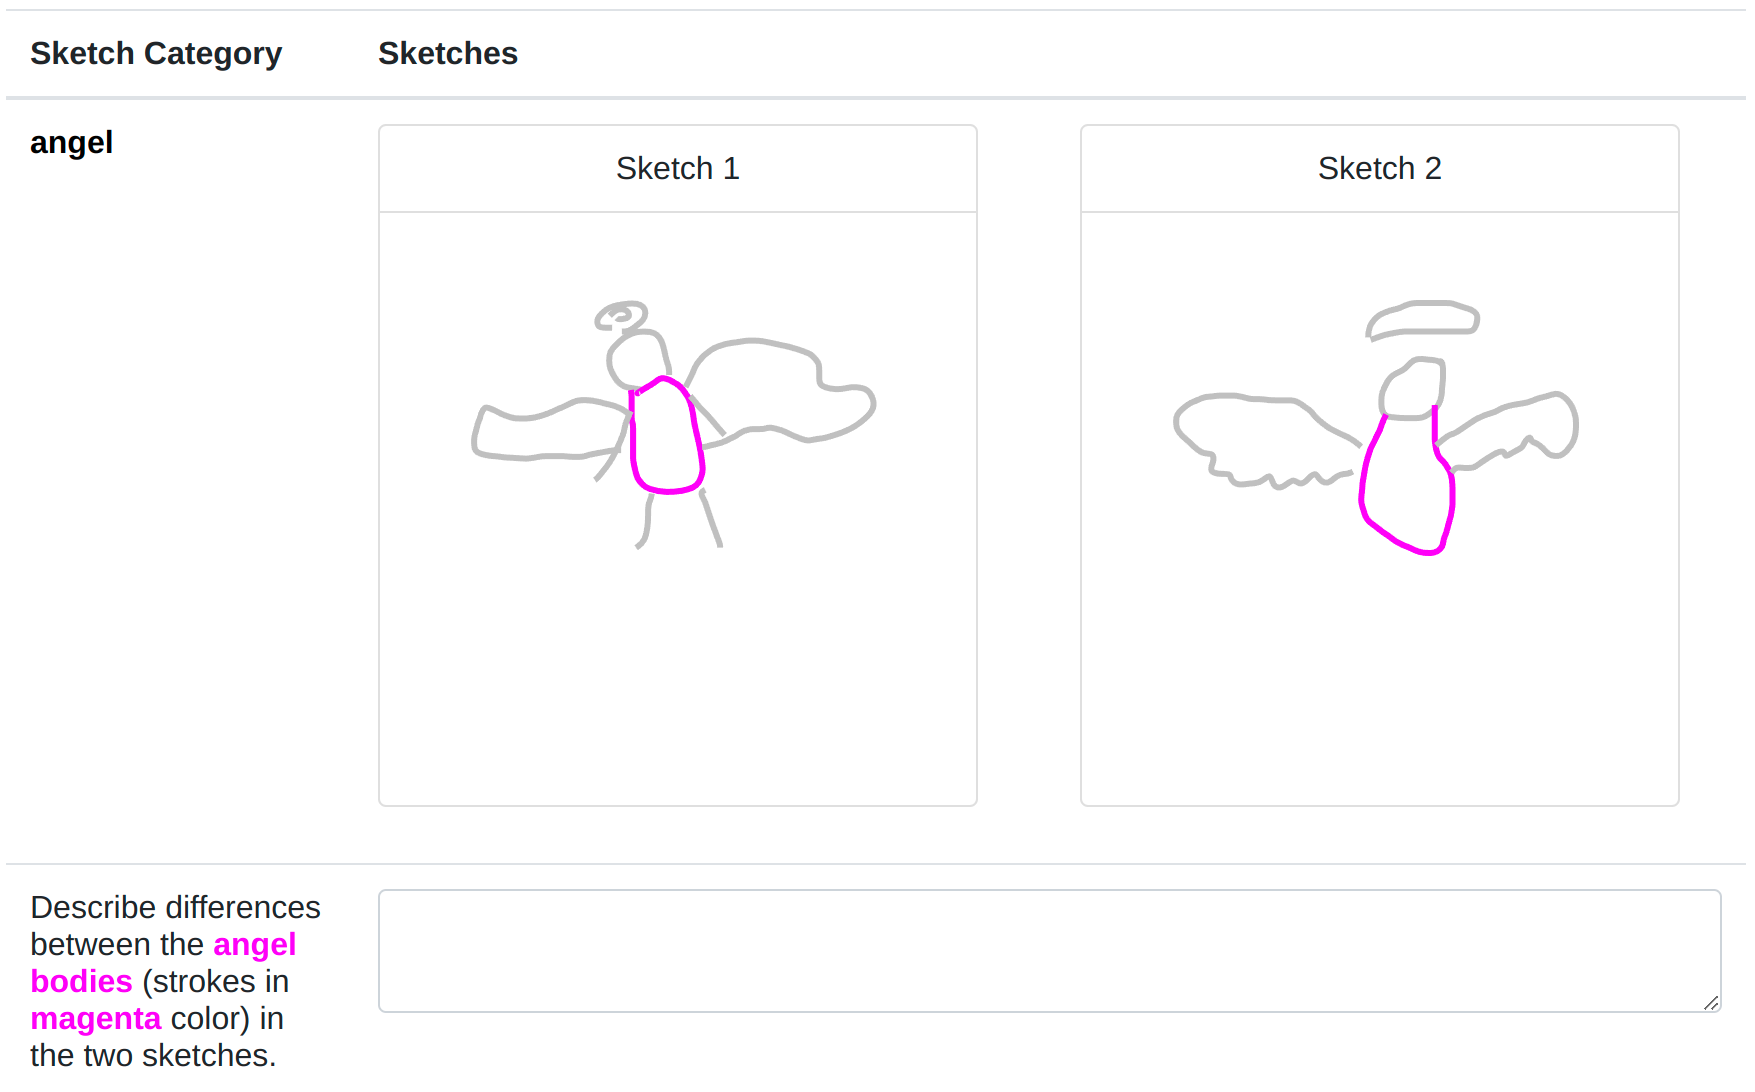
\includegraphics[width=.8\linewidth]{data_collection/version2/v2annofeb1.png}  
\caption{In the first pilot, we ask annotators to describe differences between the two sketches in full sentence.}
\label{v2.main_task.1.a}
\end{subfigure}
\newline
\begin{subfigure}{\textwidth}
\centering
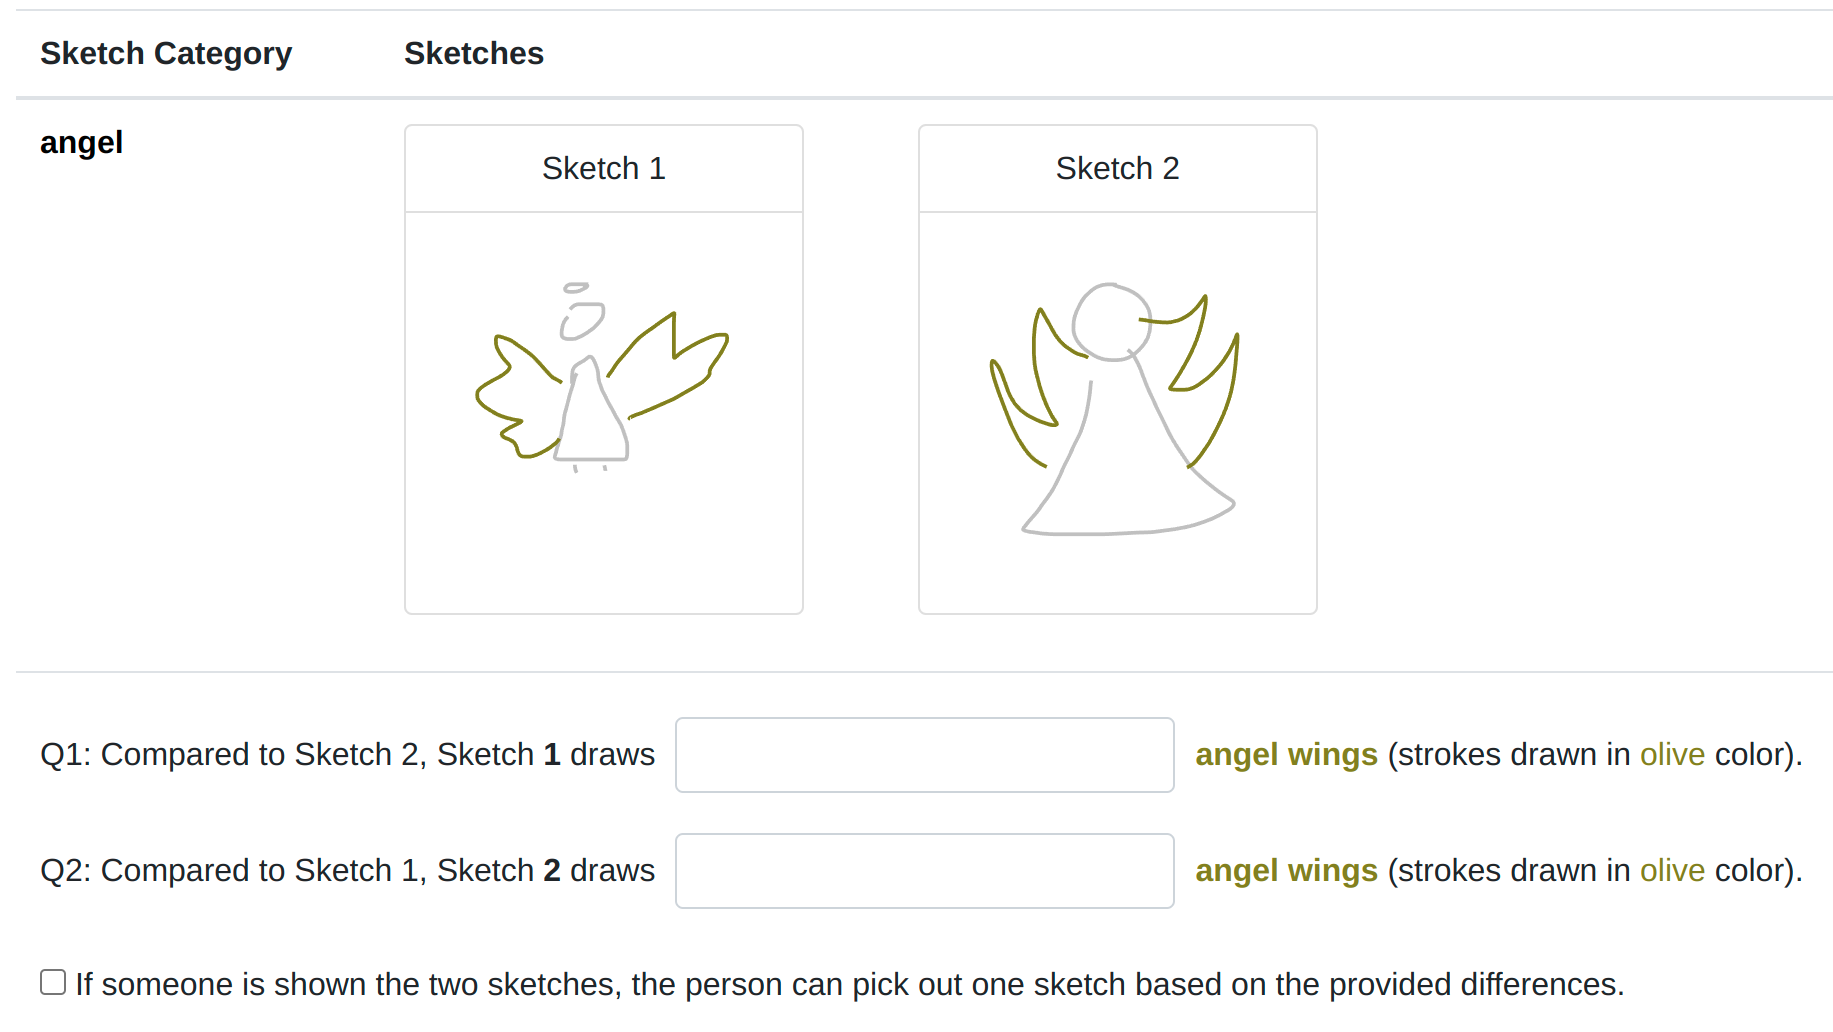
\includegraphics[width=.8\linewidth]{data_collection/version2/v2annofeb4.png}  
\caption{Compared to the previous pilot (\ref{v2.main_task.1.a}), we still ask explicitly the differences between the sketches but limit annotations to adjective phrases.}
\label{v2.main_task.1.b}
\end{subfigure}
\end{figure*}

\begin{figure*}[!htb]
\ContinuedFloat
% \begin{subfigure}{\textwidth}
% \centering
% 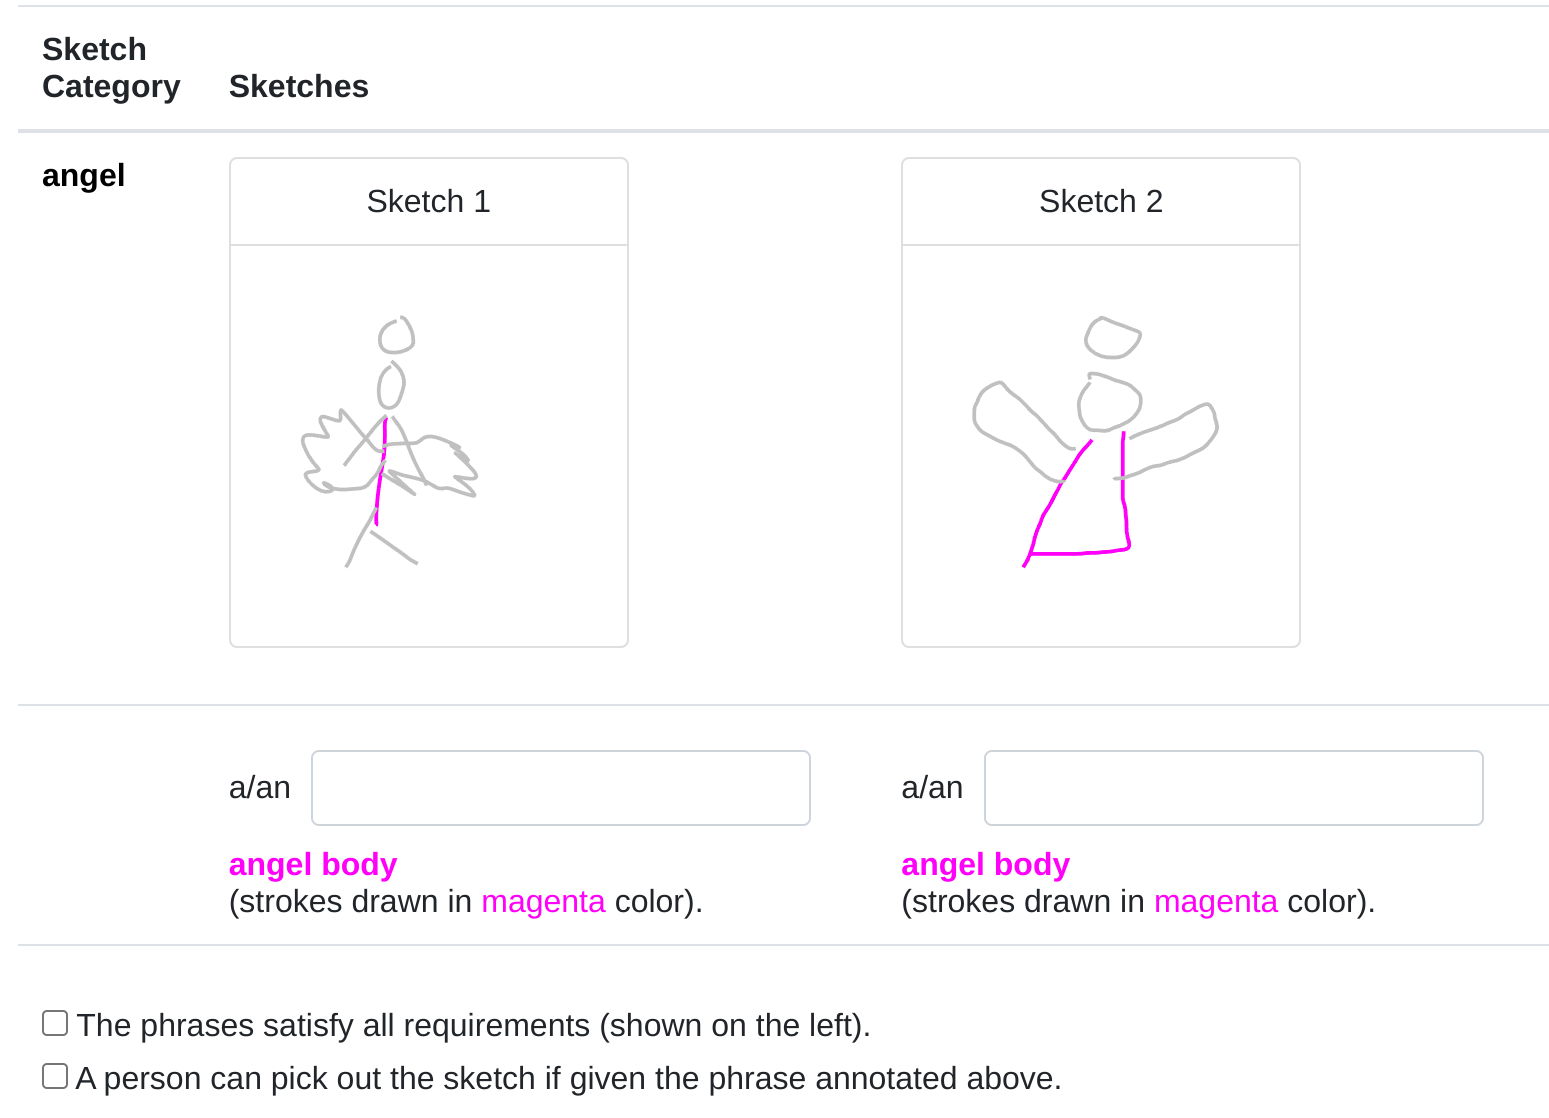
\includegraphics[width=.8\linewidth]{data_collection/version2/v2annofeb8.png}  
% \caption{Design of main task for third pilot.}
% \label{v2.main_task.1.c}
% \end{subfigure}
% \newline
\begin{subfigure}{\textwidth}
\centering
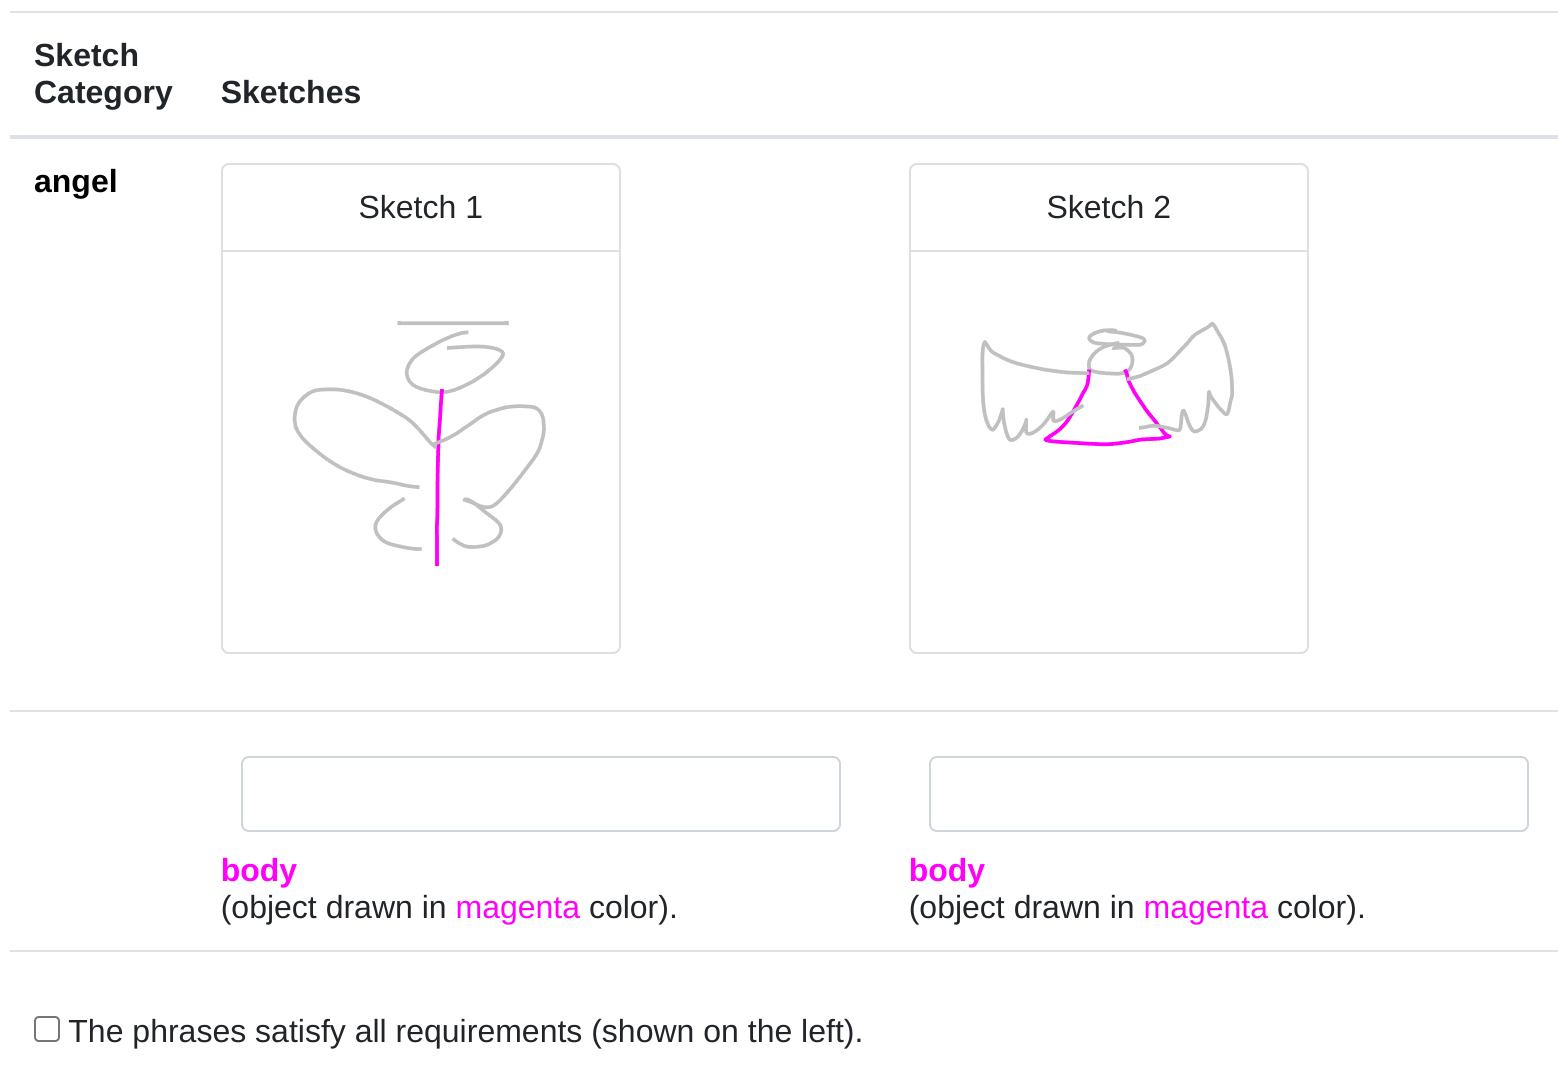
\includegraphics[width=.8\linewidth]{data_collection/version2/v2anno.png}  
\caption{Similar to the last pilot (\ref{v2.main_task.1.b}), the final version asks for adjective phrases, but we do not state explicitly that annotators should describe the visual differences to allow for more creativity.}
\label{v2.main_task.1.d}
\end{subfigure}
\caption{Different versions of the main task interface in chronological order. Final version used to collect the entire dataset is \ref{v2.main_task.1.d}.}
\label{v2.main_task.1}
\end{figure*}



\subsubsection{Main Task Interface}
When collecting the previous prompt-guided dataset, we relied on testing the interface with students in the lab to determine our design, but we observed performance differences between the students and turkers, such as amount of variety in the sketches, amount of time spent on the task, and common confusions related to understanding the requirements. 
Therefore, when collecting the contrasting sketch text dataset, we deployed several pilots on AMT to design the new interface.  
In Figure \ref{v2.main_task.1}, we show how the main task interface progressed from the first pilot to the final version used to collect the entire dataset. 

To better study how similar words are used differently across sketches, we changed to collect adjective phrases (Figure \ref{v2.main_task.1.b}, \ref{v2.main_task.1.d}) from collecting whole sentences (Figure \ref{v2.main_task.1.a}).  
We juxtaposed two sketches and highlighted the parts to be annotated in different colors to help annotators notice the contrasting features. 
Moreover, this design expedited the annotation process, since it was easier for people to perform contrasting tasks than to generate descriptions from a single sketch. 

% At the beginning, we stated explicitly that annotators should describe the differences between the sketches (\textit{Describe differences} in \ref{v2.main_task.1.a} and \textit{Compared to Sketch 1/2} in \ref{v2.main_task.1.b}), but we received many annotations that contain comparative and superlatives, so we eventually only have a blank without any introductory phrases to overly emphasize that the goal of the tasks is to create a dataset of contrastive pairs of descriptions, and the juxtaposition is meant only as a mental hint to ease annotation.

\subsubsection{Instruction and Requirement}

\begin{figure*}[!htb]
\centering
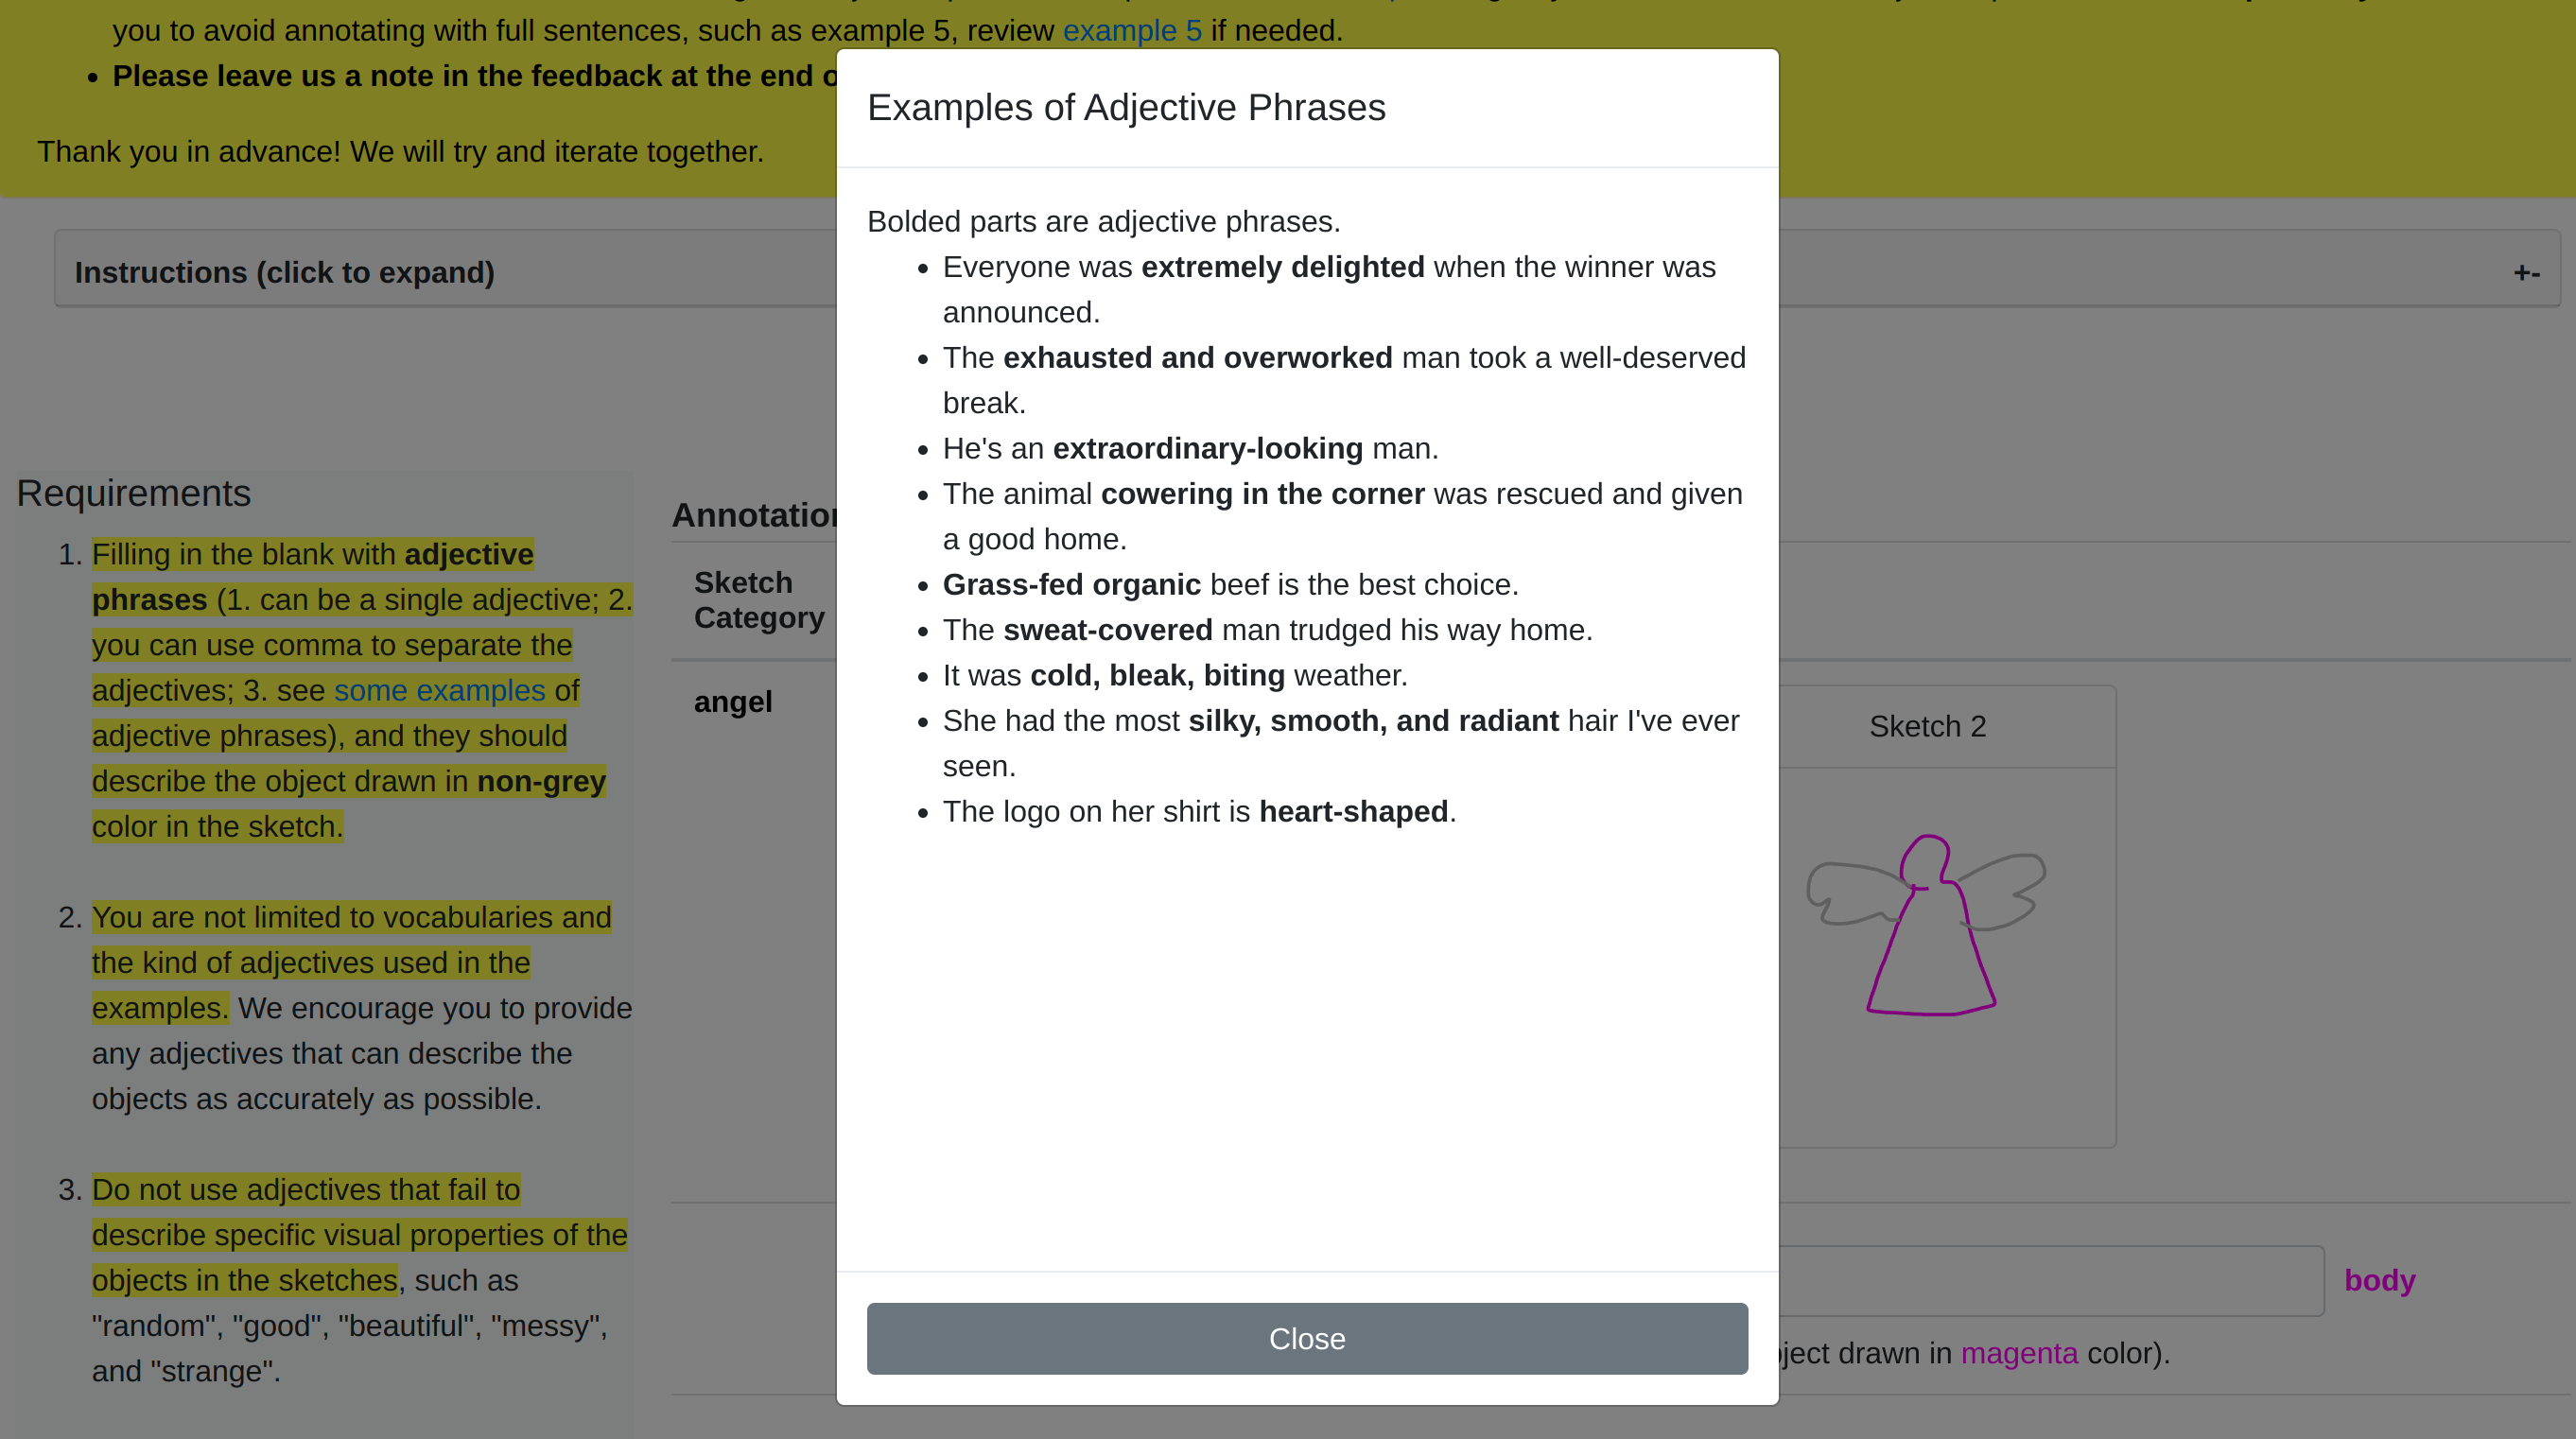
\includegraphics[width=\linewidth]{data_collection/version2/v2annoPop.png}  
\caption{A pop-up window containing examples of adjective phrases, used in collecting contrasting sketch text dataset in Section \ref{datav2}. It can be opened from the side panel by clicking on \textcolor{blue}{\it{some examples}}. Note that we used examples that are unrelated to our task on purpose, because annotators tended to repeat words in examples, so we tried to not bias them.}
\label{v2.adjective.phrases}
\end{figure*}

At the beginning, the instruction limited the annotators to provide three types of descriptions: shape, size, and position. 
However, in order to collect creative descriptions, we lifted restrictions on the type of words and only required annotators to fill in the blank with adjective phrases. We also provided some examples of adjective phrases in common sentences, unrelated to our task, for annotators to better understand their usage (Figure \ref{v2.adjective.phrases}). 

Since we simplified the HIT from 3 sub-tasks, sketching for the prompt, segmenting the sketches, and describing each step, to only asking for part descriptions, the requirements are much easier to write. 
We received less feedback from the annotators on being confused about the kind of sketches we wanted and the definition of semantic parts, which are now automatically highlighted in the sketches.   

\begin{figure*}[!htb]
\centering
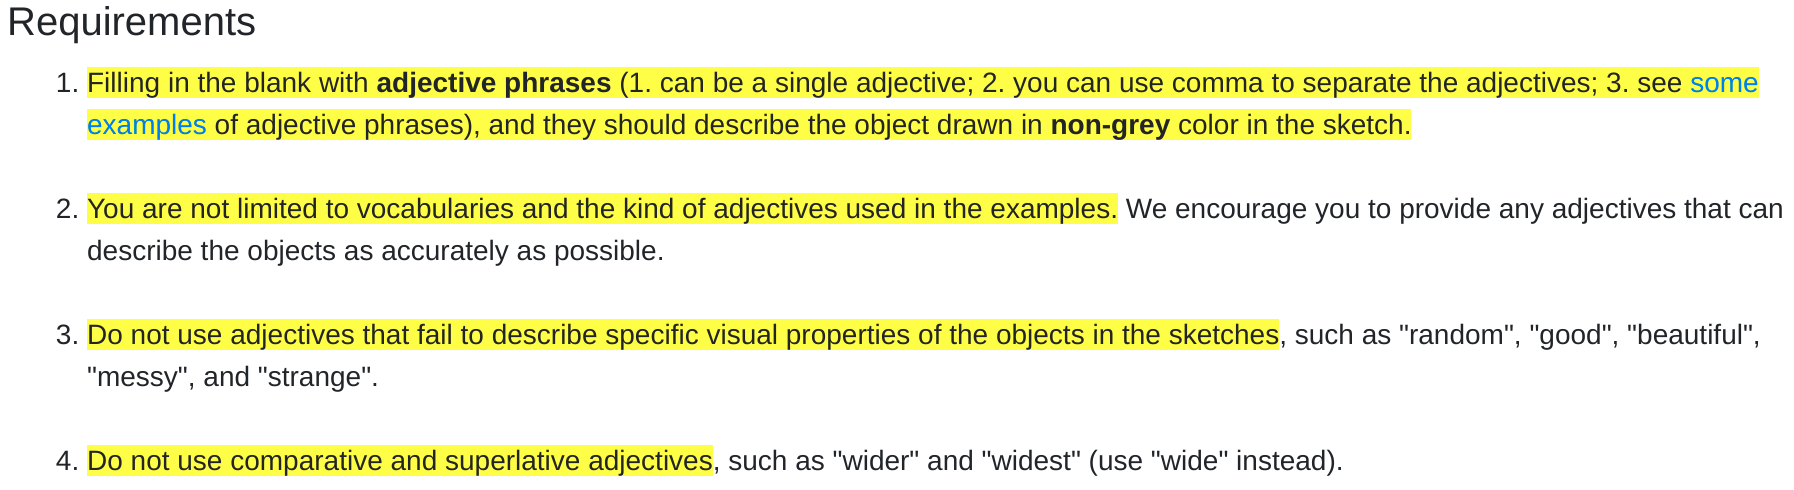
\includegraphics[width=\linewidth]{data_collection/version2/v2requirement.png}  
\caption{Requirements used in collecting the contrasting sketch text dataset (Section \ref{datav2}).}
\label{v2.requirement.1}
\end{figure*}

\begin{figure*}[!htb]
\begin{subfigure}{\textwidth}
  \centering
  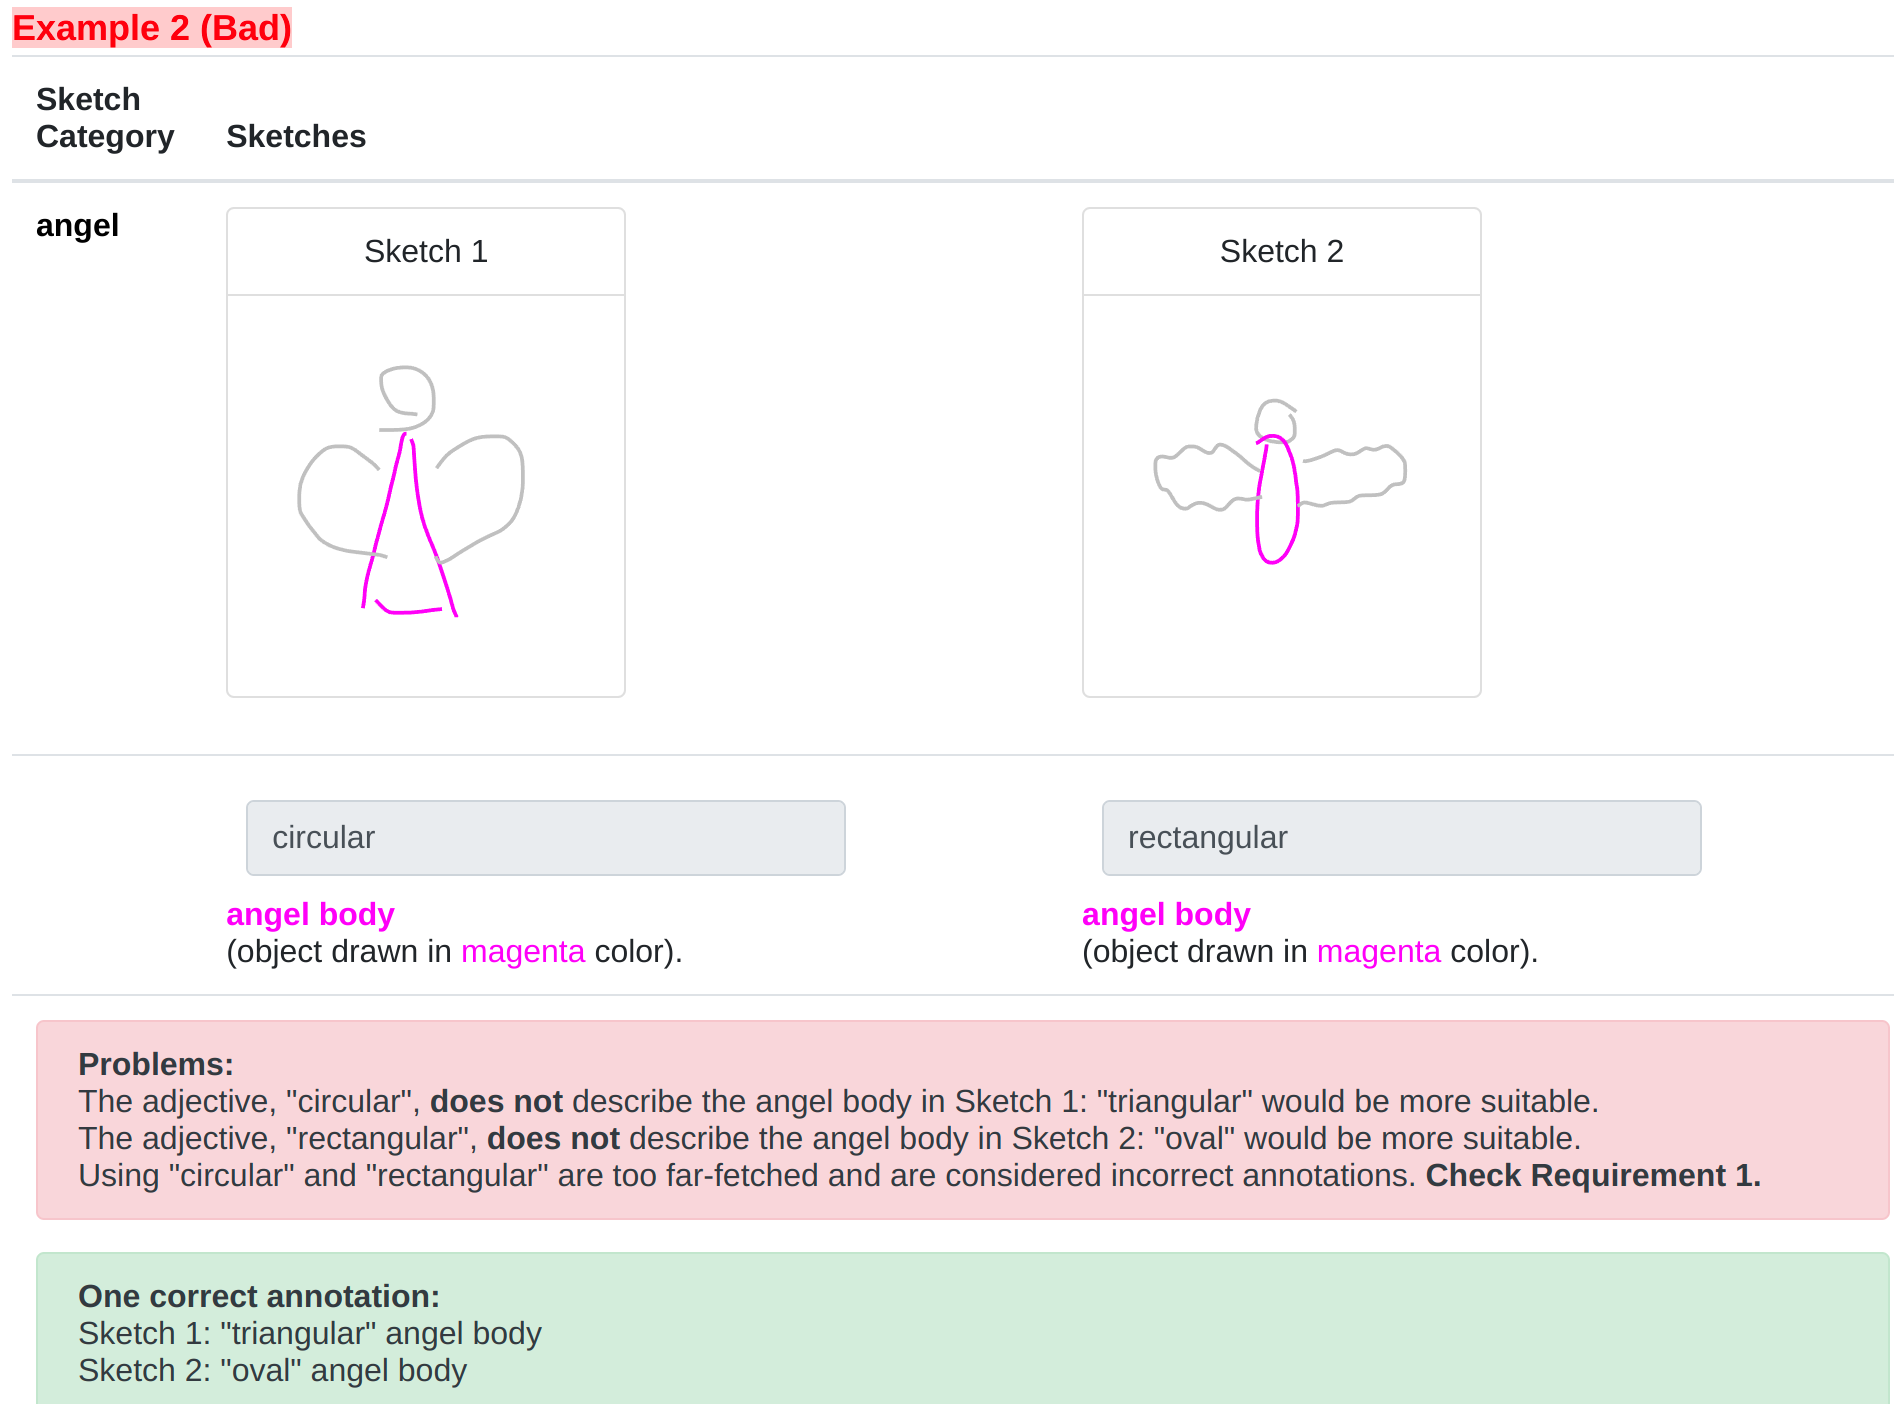
\includegraphics[width=0.8\linewidth]{data_collection/version2/v2example2.png}  
\end{subfigure}
\newline
\vspace{5mm}
\begin{subfigure}{\textwidth}
  \centering
  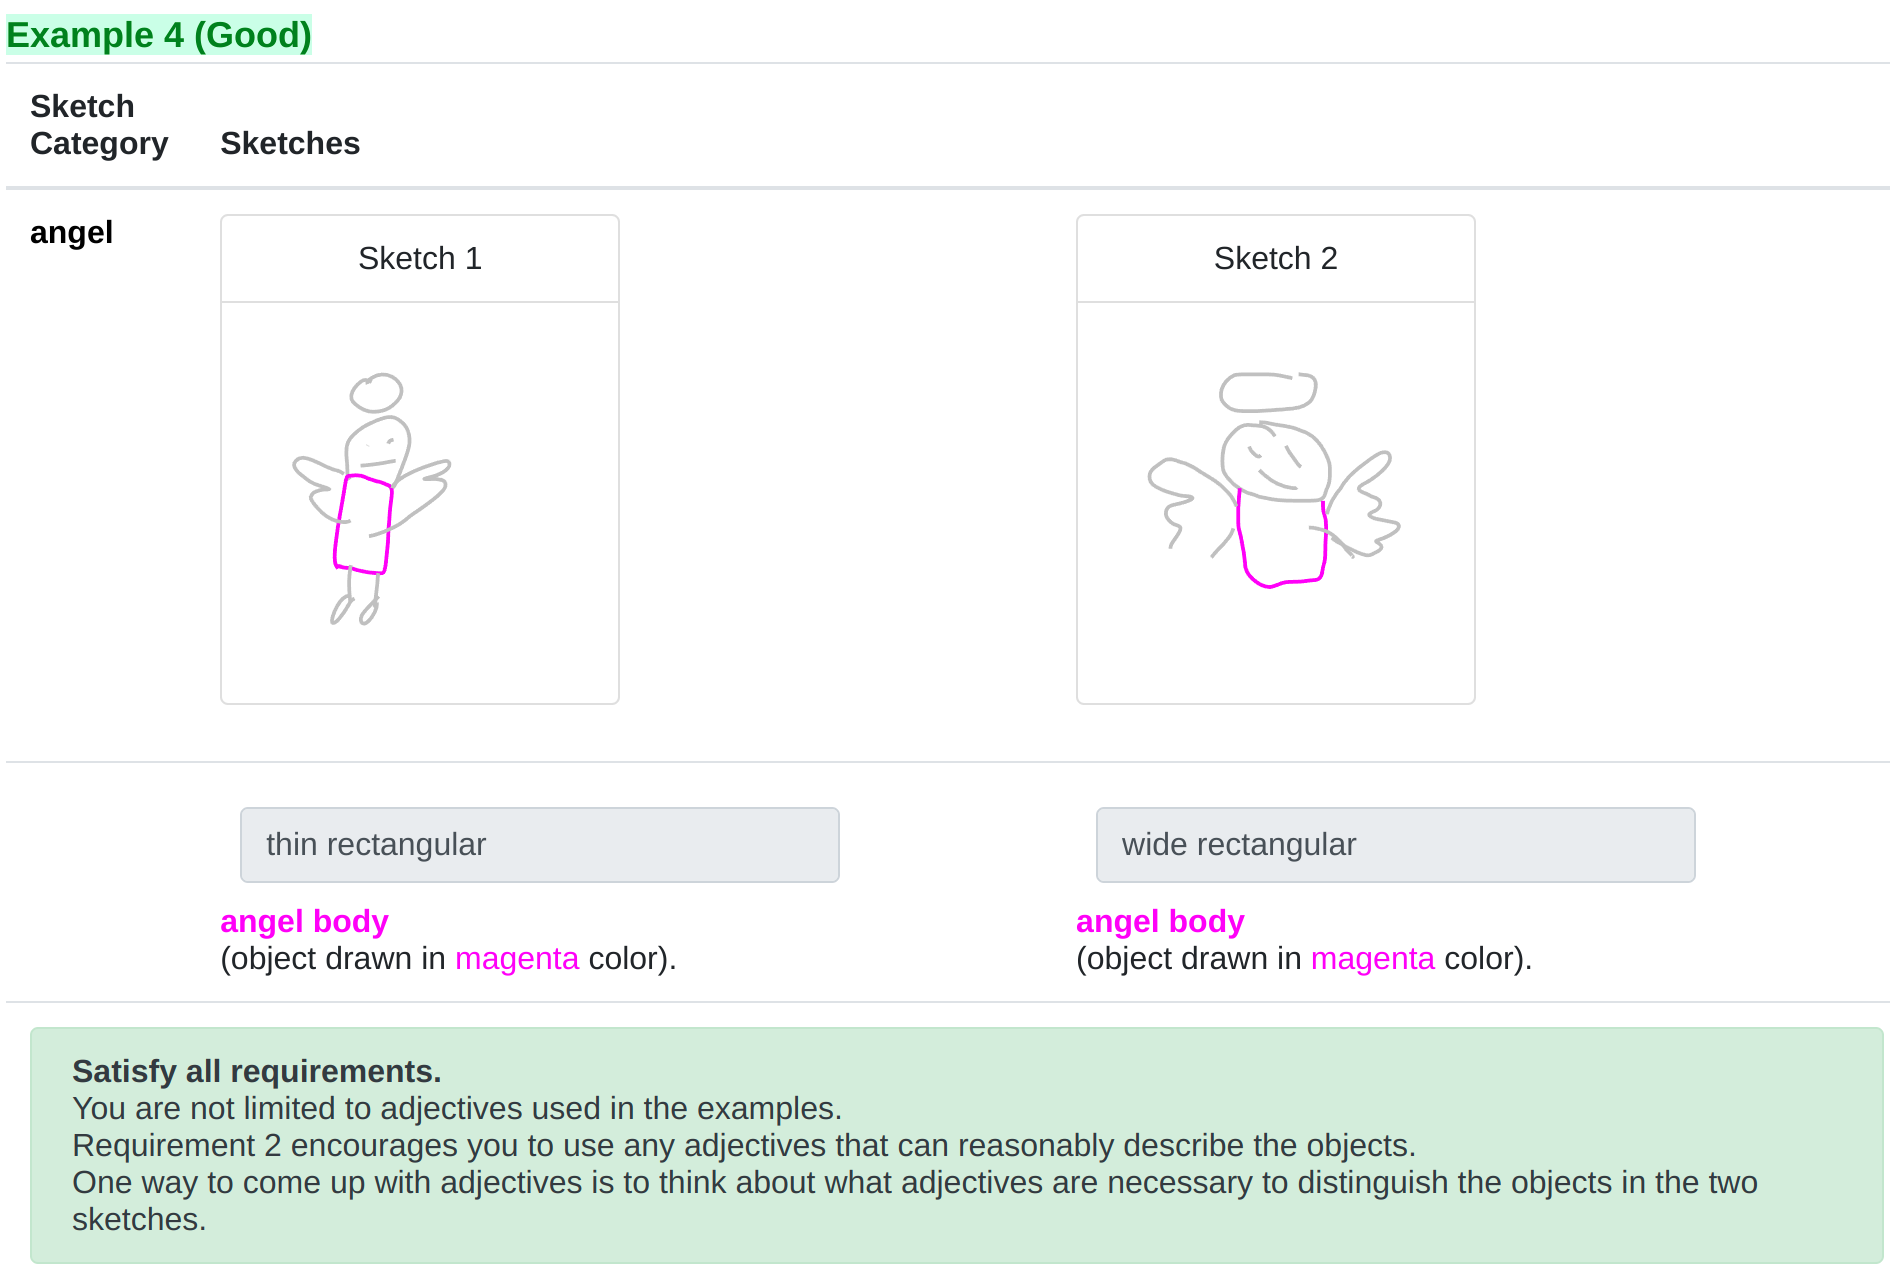
\includegraphics[width=0.8\linewidth]{data_collection/version2/v2example1.png}  
\end{subfigure}
\caption{2 examples used in the instructions to collect the contrasting sketch text dataset (Section \ref{datav2}).}
\label{v2.examples}
\end{figure*}

We relied on the examples in the instruction to give annotators an idea of what descriptions we wanted. 
Some examples that we used in the tasks are shown in Figure \ref{v2.examples}.
However, the downside was that, primed by the examples, annotators described the parts using words in the examples instead of coming up with a variety of descriptors, and we observed this behavior in the pilots. 
Therefore, we emphasized an additional requirement that asked the annotators to not limit themselves to words in the examples, and they should use any words that could illustrate the parts well. 

% The requirement that was a bit challenging for people to understand was the one regarding
% \textit{Do not use adjectives related to personal opinions, such as random, good, messy, beautiful, and strage, that are hard to achieve consensus if others were to validate your answers}. 
Since in the future we want to use our dataset to learn models that can generate sketch parts from text descriptions, the text should pertain to visual properties of the parts, so we required that \textit{Do not use adjectives that fail to describe specific visual properties of the objects in the sketches}. 
A caveat was that some annotators might consider descriptions about emotions expressed in the sketches unrelated to visual properties, since they are abstract compared to words like \textit{rectangular} and \textit{large}. 
We wanted to collect annotations for face sketches, and parts like \textit{eyes} and \textit{mouth} can be \textit{smiley} or \textit{sad}, so we added that adjectives describing emotions were allowed. 

The requirements used in the final version is shown in Figure \ref{v2.requirement.1}.

% \begin{figure*}[!htb]
% \begin{subfigure}{0.5\textwidth}
%   \centering
%   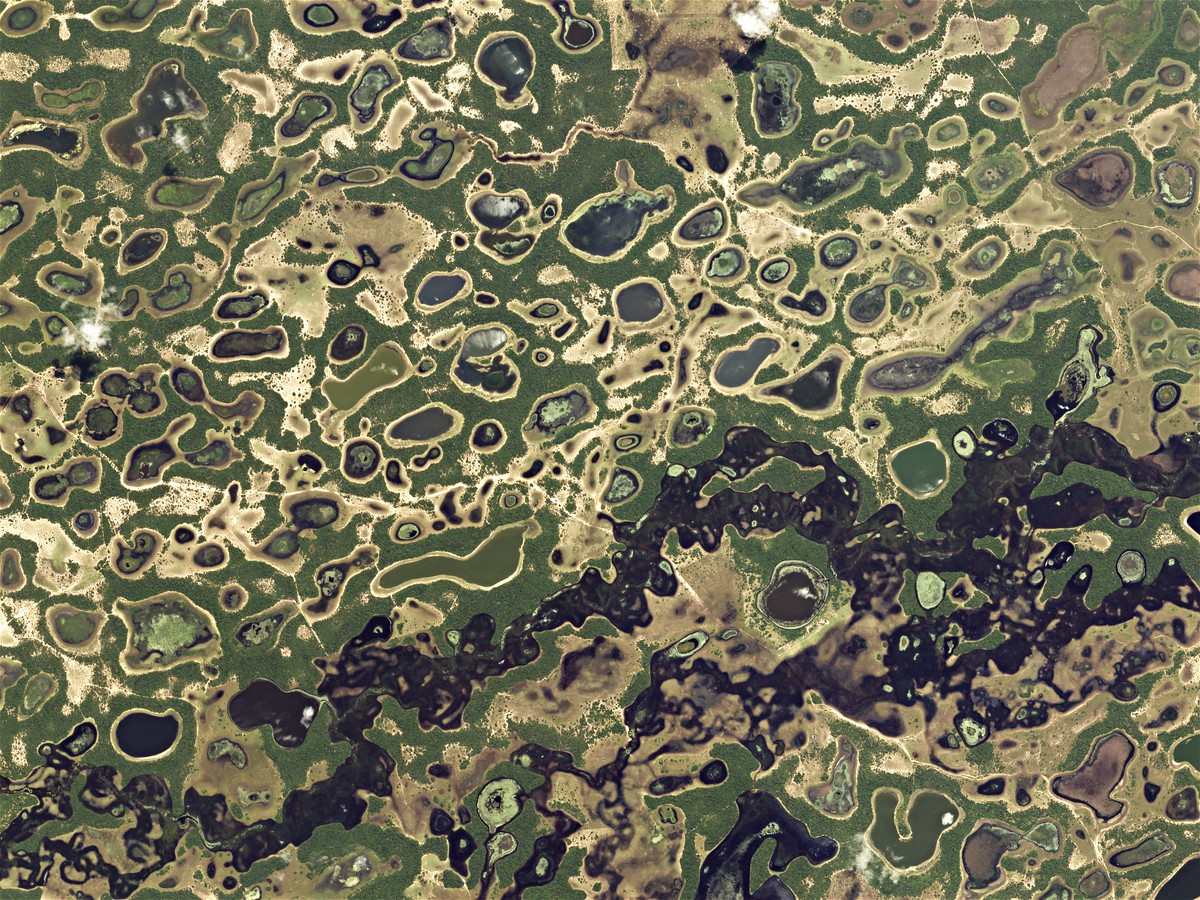
\includegraphics[width=.8\linewidth]{pantanal.jpeg}  
%   \caption{Design of main task for first pilot.}
%   \label{v2.requirement.examples.1}
% \end{subfigure}
% \begin{subfigure}{0.5\textwidth}
%   \centering
%   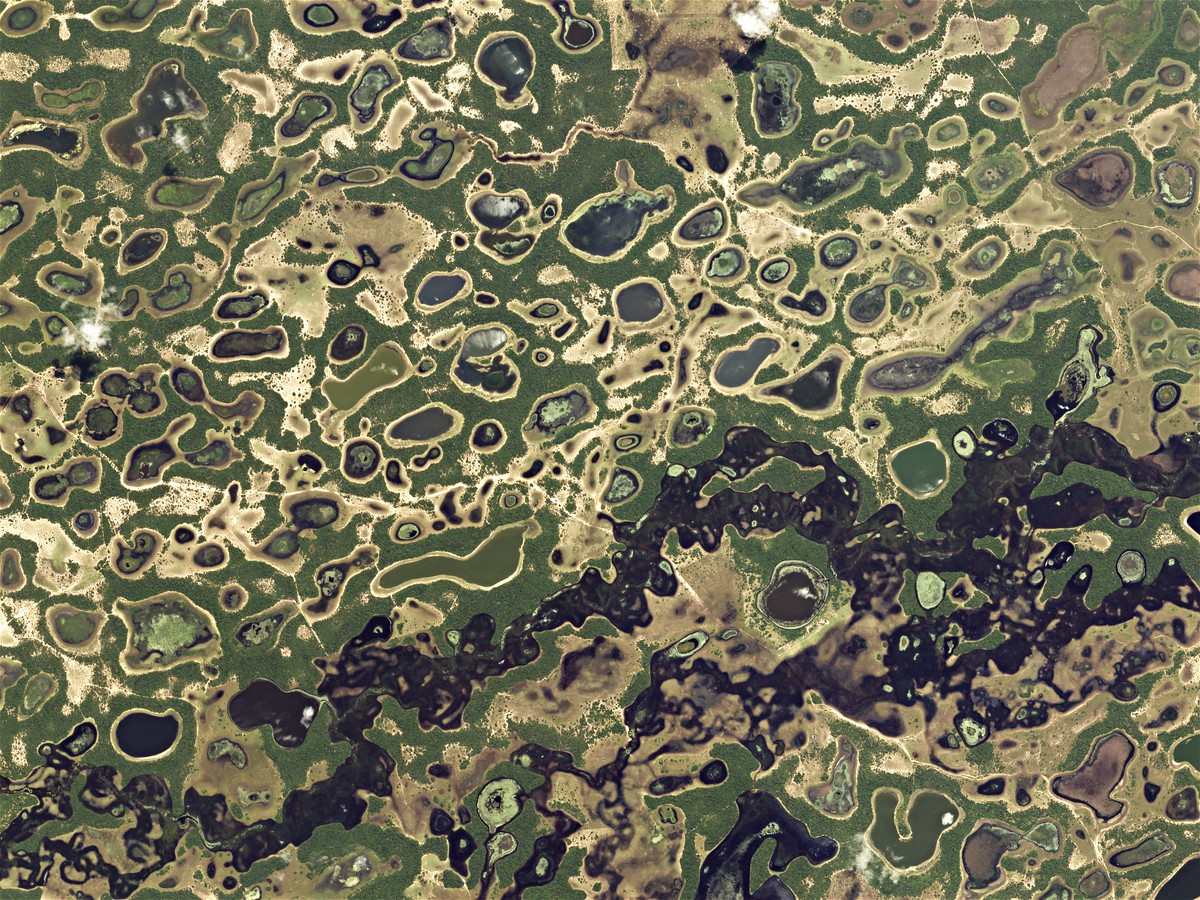
\includegraphics[width=.8\linewidth]{pantanal.jpeg}  
%   \caption{Design of main task for first pilot.}
%   \label{v2.requirement.examples.2}
% \end{subfigure}
% \newline
% \begin{subfigure}{0.5\textwidth}
%   \centering
%   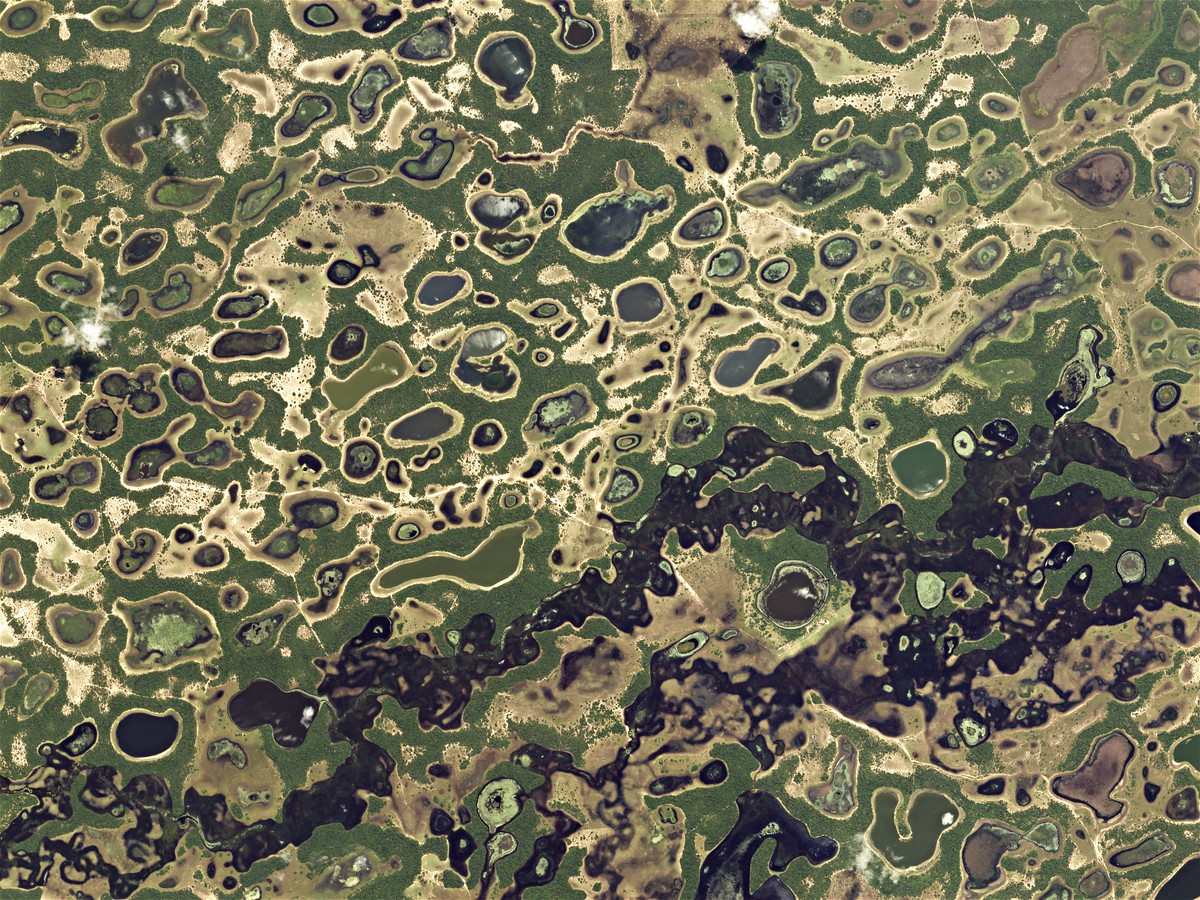
\includegraphics[width=.8\linewidth]{pantanal.jpeg}  
%   \caption{Design of main task for second pilot.}
%   \label{v2.requirement.examples.3}
% \end{subfigure}
% \begin{subfigure}{0.5\textwidth}
%   \centering
%   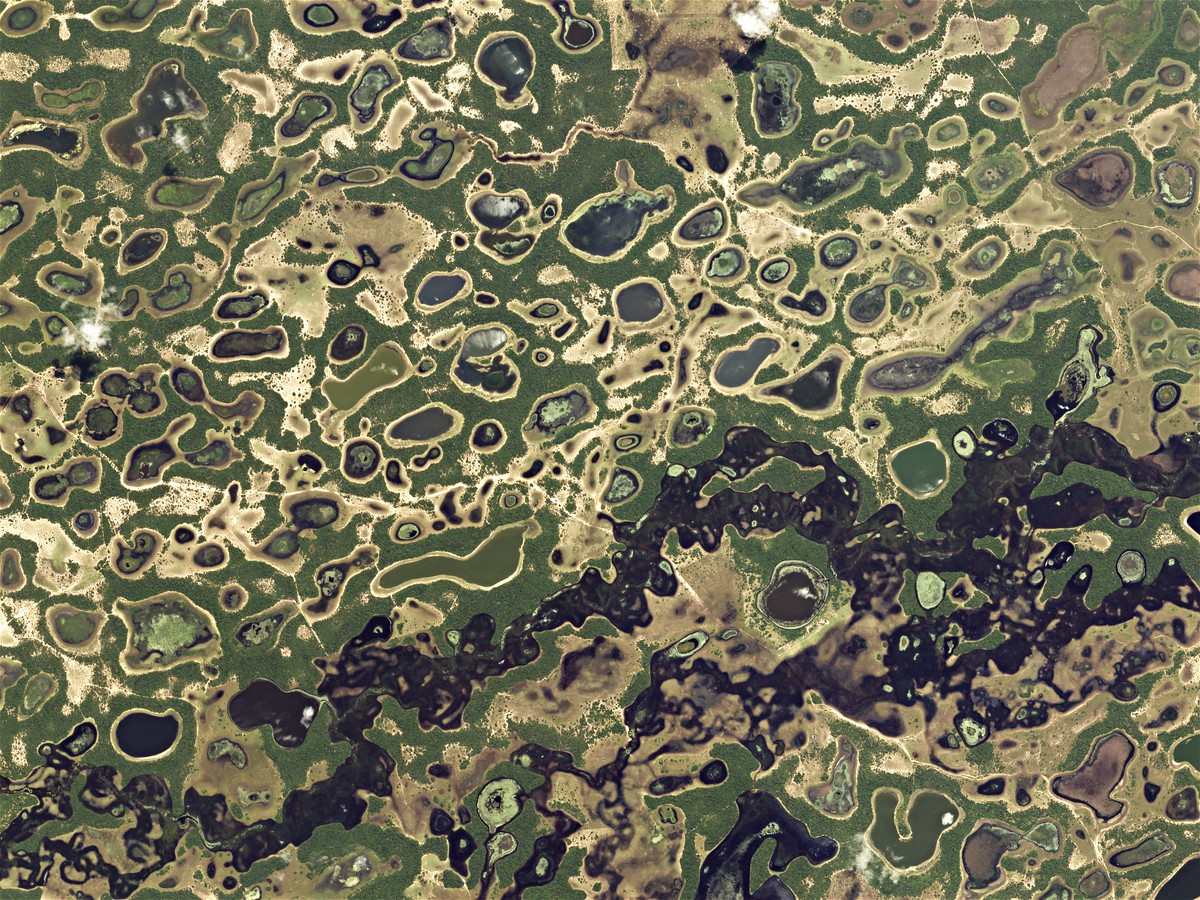
\includegraphics[width=.8\linewidth]{pantanal.jpeg}  
%   \caption{Design of main task for second pilot.}
%   \label{v2.requirement.examples.4}
% \end{subfigure}
% \newline
% \begin{subfigure}{0.5\textwidth}
%   \centering
%   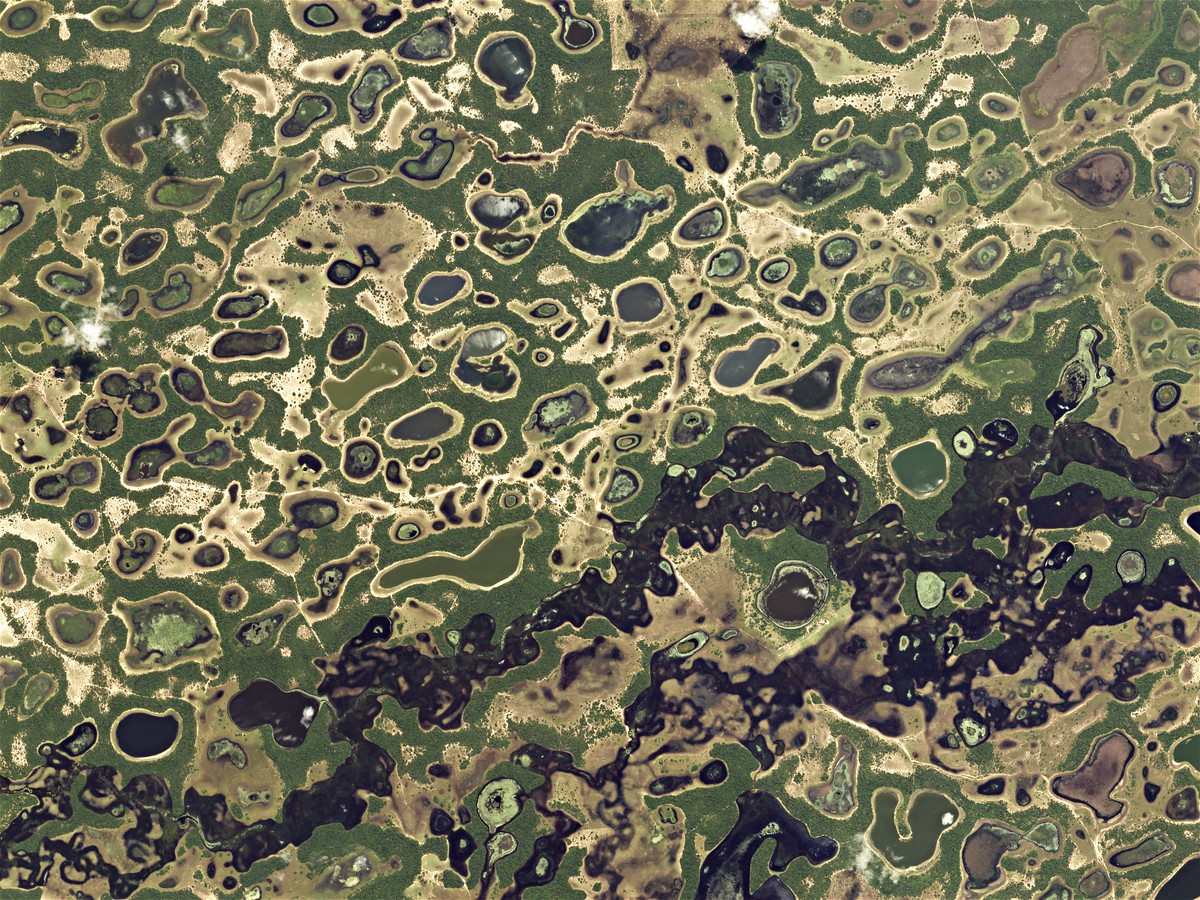
\includegraphics[width=.8\linewidth]{pantanal.jpeg}  
%   \caption{Design of main task for second pilot.}
%   \label{v2.requirement.examples.5}
% \end{subfigure}
% \begin{subfigure}{0.5\textwidth}
%   \centering
%   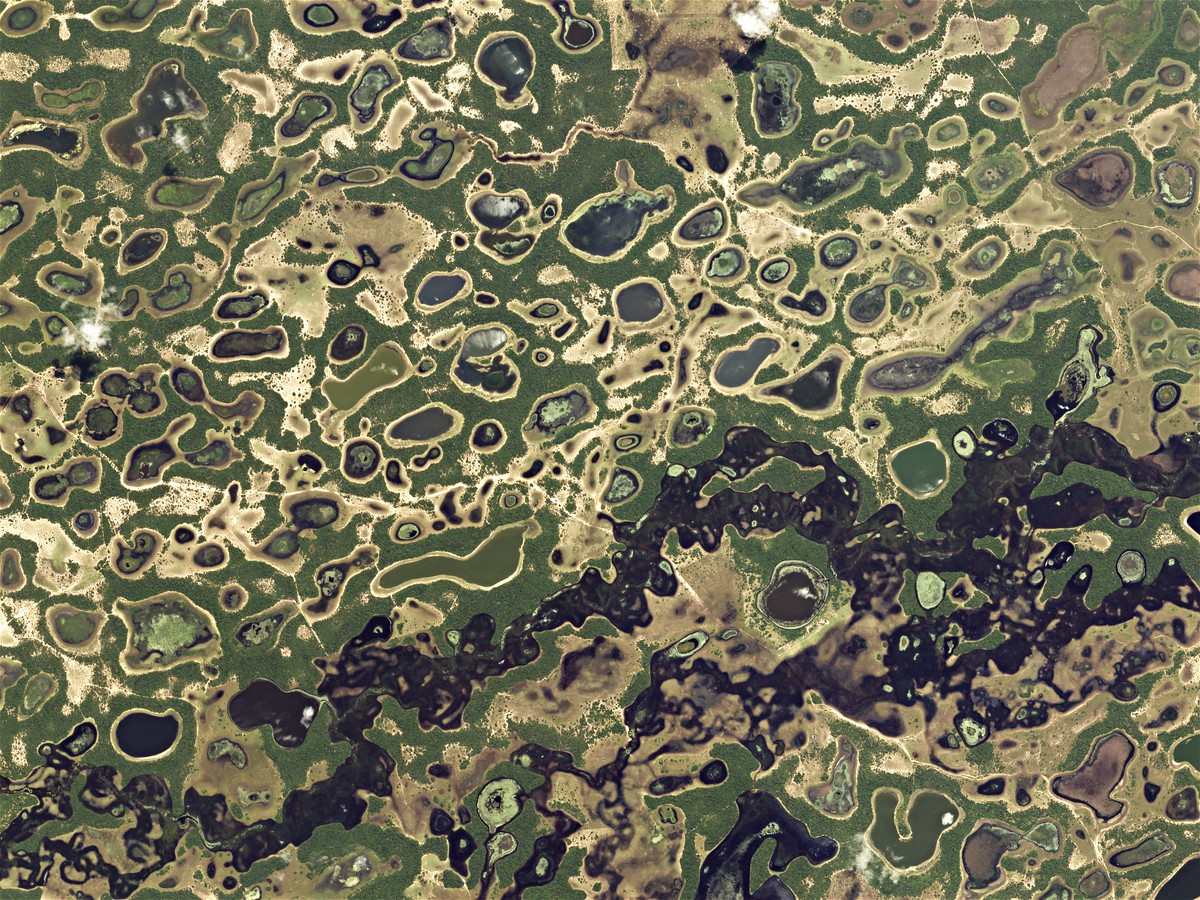
\includegraphics[width=.8\linewidth]{pantanal.jpeg}  
%   \caption{Design of main task for second pilot.}
%   \label{v2.requirement.examples.6}
% \end{subfigure}
% \caption{Progress of the design two for the main task in version two.}
% \label{v2.requirement.examples}
% \end{figure*}





\subsubsection{Qualification}
We prepared 10 qualification questions; all are yes/no questions.
We used the qualification test to train turkers to understand the requirements better. 
Each question had a hint that stated which requirement and examples were helpful for solving the question. The purpose of the qualification test was not to trick annotators but to ensure speed and quality of the annotation. 
We show one question from the qualification in Figure \ref{v2.qualification.1}. 
To see the full test, refer to: \url{https://erinzhang1998.github.io/portfolio/v2qual}. 
At the end, we recruited 88 annotators to work on our task. 

\begin{figure*}[!htb]
\centering
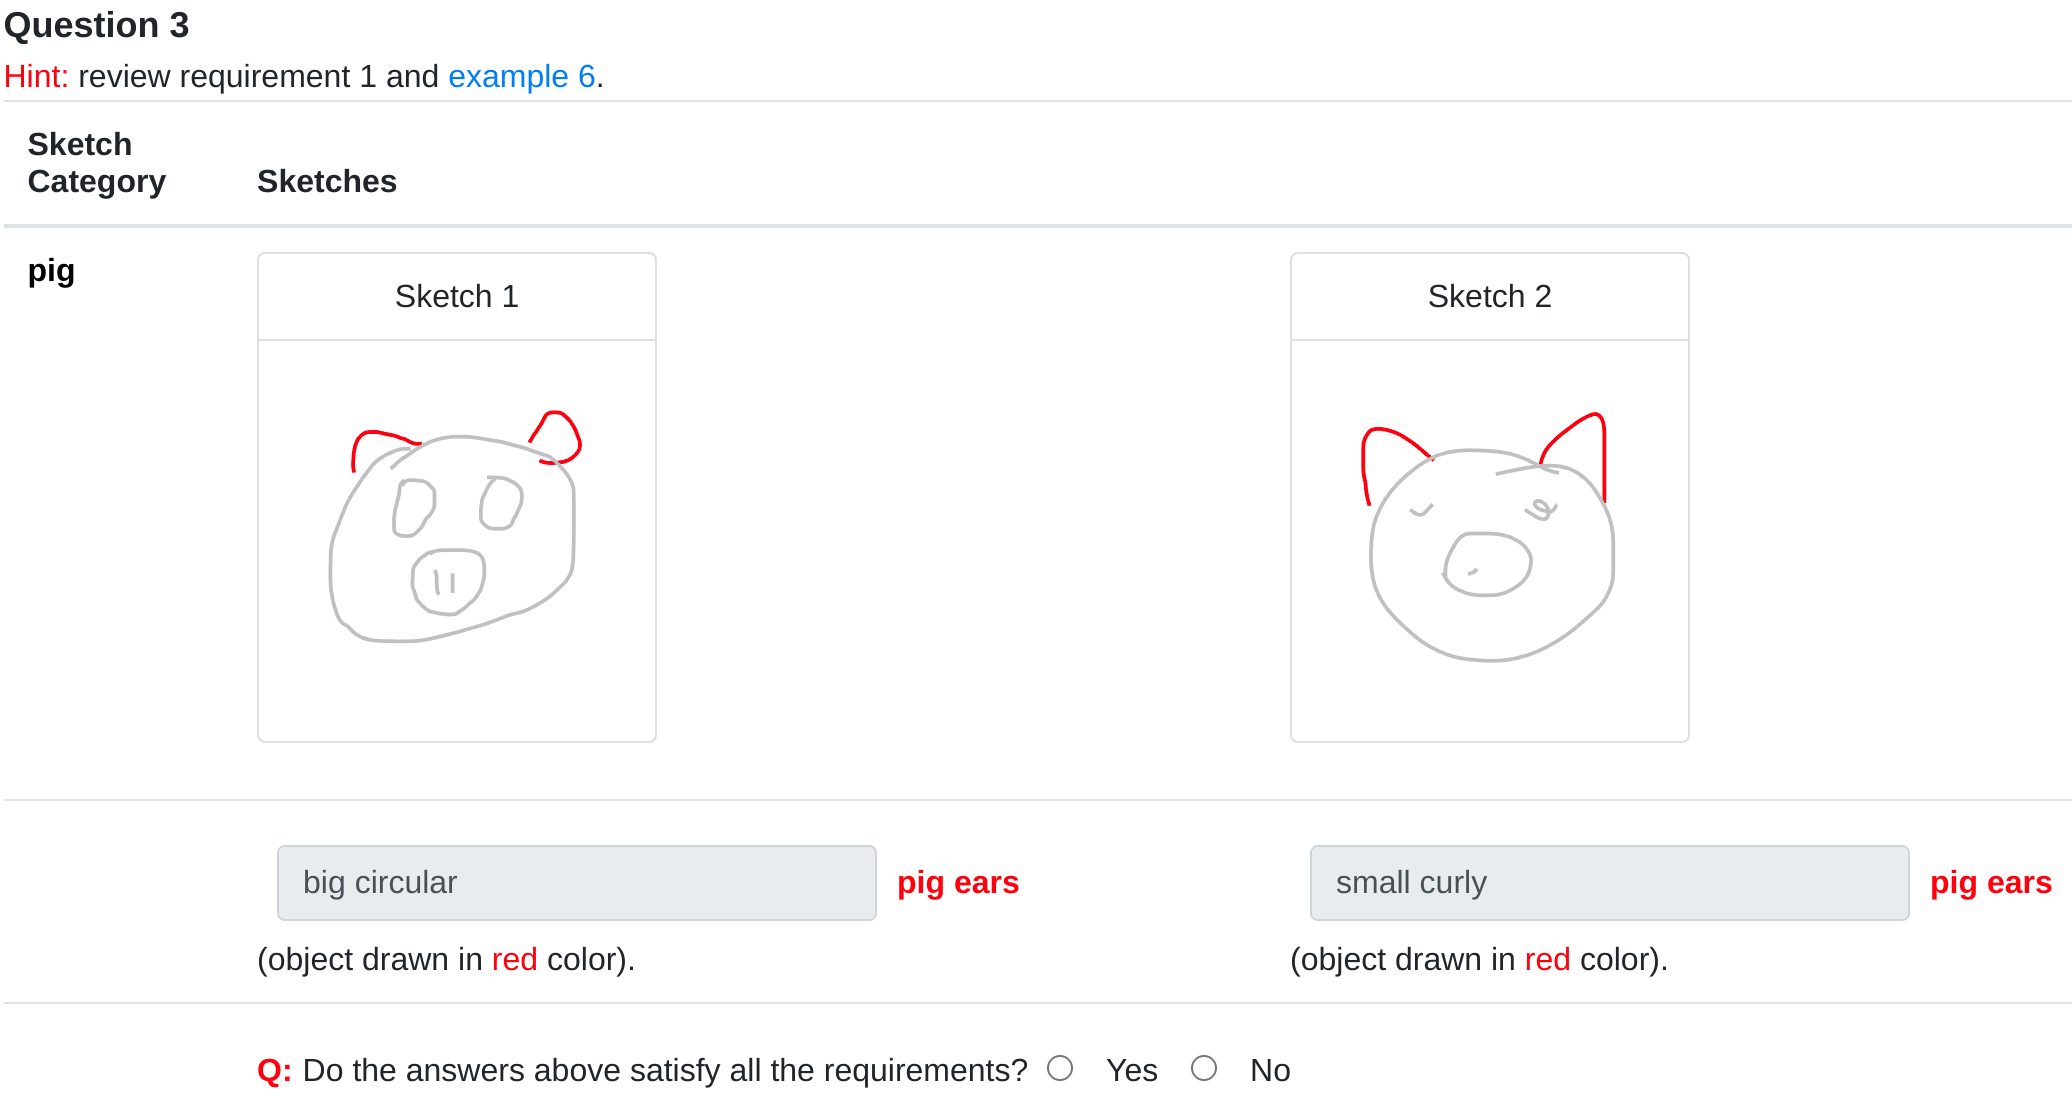
\includegraphics[width=\linewidth]{data_collection/version2/v2qualQ3.png}  
\caption{Question 3 from the qualification test used to collect the contrasting sketch text dataset (Section \ref{datav2}). We show a hint at the beginning of each question telling the annotators which requirement this question is testing. In this way, we encourage them to review the requirements so that they have a good understanding of the task and can provide high-quality annotations in the real HIT. The question interface is the same as main task interface that annotators will see when they annotate. The 1-to-1 mock-up helps them to be familiar with the workflow.}
\label{v2.qualification.1}
\end{figure*}

% \begin{table*}[!htb]
% \begin{minipage}[b]{1\textwidth}
% \centering
% \begin{tabular}{l|rrrrrrrrrr}
% \toprule
% Question Number  & 1 & 2 & 2 & 2 & 2 & 2 & 2 & 2 & 2 & 2  \\
% Correct Rate  & 1 & 2 & 2 & 2 & 2 & 2 & 2 & 2 & 2 & 2\\
% \bottomrule
% \end{tabular}
% \caption{Success rate of each question in the qualification test}
% \label{v2.qualification.success_rate}
% \end{minipage}
% \end{table*}
% We released $n$ copies of qualifications, and $n_2$ annotators scored $90$ or higher. The average score for the entire test is $x$, and the rate of correct answer for each question is shown in Table \ref{v2.qualification.success_rate}. Before releasing the qualification, we have tested the test on 



\subsection{Results}

\subsubsection{Pilot 1}
In order to work out the data collection process, we chose the angel category and try to manually examine the sketches and categorize them based on 


One purpose of the pilot is to estimate the amount of money that we need to spend for each task, and from Table \ref{v2.workertime}, we see that []
\begin{table*}[!htb]
\begin{minipage}[b]{1\textwidth}
\centering
\begin{tabular}{l|rrrrr}
\toprule
~ & Max. & Min. & Mean & Med. & Std. \\
\midrule
Feb 01 Pilot  & 1 & 2 & 2 & 2 & 2   \\
Feb 04 Pilot  & 1 & 2 & 2 & 2 & 2  \\
Feb 08 Pilot  & 1 & 2 & 2 & 2 & 2  \\
Official Collection  & 1 & 2 & 2 & 2 & 2  \\
\bottomrule
\end{tabular}
\caption{Comparing time statistics of pilot task}
\label{v2.workertime}
\end{minipage}
\end{table*}

For the data collection process, we decide to collect for the face category of the QuickDraw dataset, and the reason for it was mainly to echo the choice of many SOTA generative modeling works that are done on the CelebA dataset. It seems that face generation is quite a starting point for many of the generative modeling work. We have also surveyed some text-to-image synthesis methods that use datasets like (1) CUB dataset (2) MNIST (3) Omniglot. Several sketch datasets include the one from DoodlerGAN and SketchBirds. A lot of the datasets focus on one or two categories, so we decide to do the same to ensure that with our budge, we can collect a dataset that contains enough signal to train a generative ML model. 

Clustering the faces, we strive to present to the annotators pairs of faces that are distinct as possible in order help them to provide good annotations. It is easier for them to grasp and understand the features of the objects if two sketches are presented in a contrasting way. 



If we use CLIP to extract the visual features for the entire face sketch.

